% Project overview: motivation and work to date (UMU-Bench track).
% Numbers come from DEVIATIONS.md (DEV-011 to DEV-013) and from the figures in figures/.
% Compile from this directory: pdflatex overview.tex (run twice for references).
\documentclass[11pt]{article}
\usepackage[margin=1in]{geometry}
\usepackage[T1]{fontenc}
\usepackage{lmodern}
\usepackage{microtype}
\usepackage{amsmath,amssymb}
\usepackage{booktabs}
\usepackage{tabularx}
\usepackage{enumitem}
\usepackage{xcolor}
\usepackage{graphicx}
\usepackage[colorlinks=true,linkcolor=black,citecolor=black,urlcolor=blue!50!black]{hyperref}
\setlist{itemsep=2pt,topsep=4pt}
\newcommand{\thu}{\theta_u}
\newcommand{\tho}{\theta_0}
\newcommand{\Hp}{H1$'$}
\newcommand{\dwx}{$\lVert\Delta W x\rVert$}

\title{Text-Only Unlearning in a Vision--Language Model:\\
Motivation and Work to Date}
\author{Xuzhong Wang}
\date{Project overview --- 19 November 2026}
\begin{document}
\maketitle

\section{Summary}
We remove facts about fictitious people from a vision--language model (VLM) using text
questions only, and then ask what the unlearning changed inside the model. After
unlearning, accuracy on the forget facts falls from 1.00 to 0.63 when the question names the
person, but stays at 0.97 when the question shows the person's portrait. Interventions on
the unlearned model show three things. The knowledge is still in the model. The update
that causes the forgetting sits in decoder layers 0--19 and acts across the whole text
prompt, not on the name alone. Adding an image to the name question, even a blank one,
removes most of the suppression. A final test swaps what the unlearning adapter writes
between the two prompts: the adapter writes nearly the same thing with and without the
image, and the answer is suppressed only when those writes land in a text-only prompt. Our
current reading is that text-only unlearning teaches the model to suppress answers to one
\emph{form of input}; it does not remove what the model knows about a person. All
mechanism results come from one checkpoint of one run.

\section{Motivation}
\paragraph{The problem.} Machine unlearning tries to make a trained model behave as if it
had never learned certain facts, for example personal data that must be deleted. In a VLM
the same fact can be reached through two kinds of input: a text question that names the
person, or a question about the person's portrait. Several benchmarks report that
unlearning through one kind of input leaves the fact answerable through the other
\cite{umubench,unlinkvl,smu,idunlearn}. A model that has ``forgotten'' a person in text
but still answers from a photo has not forgotten the person.

\paragraph{The gap.} The explanations offered so far have not been tested by intervening
on the unlearned model. CrossInf reports internal measures that are correlational
(per-layer LoRA magnitude and representation similarity) \cite{crossinf}. PAVA traces how
names and faces are processed, but in the model \emph{before} unlearning \cite{pava}.
UMU-Bench attributes the leak to misalignment between modalities without an internal
analysis \cite{umubench}. For text-only language models there is evidence that common
unlearning methods suppress the extraction of a fact and leave the stored knowledge in
place \cite{hong2024,guo2024}; whether the same holds in a VLM, and how it produces the
cross-modal leak, was open.

\paragraph{Our question.} After text-only unlearning, why does the portrait question still
get the answer? We started from three candidate mechanisms, written down before any
mechanism experiment (Table~\ref{tab:hyp}).

\begin{table}[htbp]
\centering\small
\begin{tabularx}{\linewidth}{@{}lXX@{}}
\toprule
 & Claim & What it predicts\\
\midrule
H1 & Unlearning adds a suppression in the late layers that only features of the text
route trigger. & Removing the update from the late layers restores the answer to the name
question.\\
\Hp & Unlearning changes how the early layers process the name tokens; the portrait route
identifies the person elsewhere and never passes through the change. & The update is
concentrated on the name tokens in the early layers.\\
H2 & The portrait route is suppressed as well, but later layers restore the answer. &
Under the portrait question, the answer probability dips in the middle layers and then
recovers.\\
\bottomrule
\end{tabularx}
\caption{The three starting hypotheses.}
\label{tab:hyp}
\end{table}

\section{Setup}
\paragraph{Data and model.} UMU-Bench contains fictitious people; each fact has a
name-based text question and a portrait-based question \cite{umubench}. We use the
LLaVA-1.5-7B checkpoint that the UMU-Bench authors fine-tuned on these people and released
(\texttt{chengyewang/llava\_smu\_ft}) \cite{llava15}. This is the ``vanilla'' model
$\tho$. Its fine-tuning data attached the portrait to every item, so it never saw an input
without an image.

\paragraph{Unlearning.} We train a fresh LoRA adapter (rank 16) on the linear layers of
the language model. The forget set is 50 people. Training uses only their name-based
questions, with no image (600 question--answer pairs). The method is negative preference
optimization (NPO, $\beta=0.4$) \cite{npo}; the main run adds a retain term, the ordinary
language-model loss on name-based questions about other people. The unlearned model is
$\thu$.

\paragraph{Readout.} We score the model the way UMU-Bench does: the options are listed in
the prompt, the model generates greedily, and the answer counts as correct only if it
equals the correct option text. With this readout the vanilla scores 0.75 by name and 0.81
by portrait on the forget set and reproduces the paper's accuracy (0.823 against 0.8233).
All results below are on \emph{doubly-correct} facts, those the vanilla answers correctly
both by name and by portrait: 65 forget facts and 26 retain facts (from 20 people outside
the forget set). The leak is $G=\text{portrait accuracy}-\text{name accuracy}$ on these
facts.

\paragraph{Why this setup.} The first attempt used MLLMU-Bench \cite{mllmu} with our own
fine-tuned vanilla (Qwen2-VL-2B). It reached only 0.379 (image) and 0.439 (text) on paired
multiple-choice items, against a target of 0.80, so the facts were not reliably in the
model. Two findings from that attempt shaped the current setup. First, MLLMU-Bench's text
and image questions mostly ask about different attributes of the same person (28.4\%
overlap in the forget split), so they cannot be compared fact by fact; UMU-Bench pairs
them. Second, reading the probability of the option letter underestimates what the model
knows: on the same UMU-Bench items it gives 0.51 / 0.53 where generation gives
0.75 / 0.81.

\section{What we ran}
\subsection{Unlearning runs}
Table~\ref{tab:runs} lists the four training runs. Run~2 is the only one that forgets
without collapsing, and every mechanism analysis uses its final checkpoint (step 150).

\begin{table}[htbp]
\centering\small
\begin{tabularx}{\linewidth}{@{}lXcccc@{}}
\toprule
Run & Setting & Forget, name & Forget, portrait & $G$ & Retain, name\\
\midrule
1 & NPO only, lr $5\times10^{-5}$ (step 75) & 0.585 & 0.969 & 0.385 & 0.769\\
--- & NPO + retain, lr $2\times10^{-5}$ (step 76, stopped) & 0.985 & --- & --- & ---\\
2 & NPO + retain on 50 people, lr $5\times10^{-5}$ (step 150) & 0.631 & 0.969 & 0.338 & 0.692\\
3 & Retain weight 3 on 200 people, lr $5\times10^{-5}$ (step 150) & 0.923 & 0.969 & 0.046 & 0.962\\
\bottomrule
\end{tabularx}
\caption{Unlearning runs, scored on doubly-correct facts (all 1.00 before unlearning).}
\label{tab:runs}
\end{table}

\begin{itemize}
\item \textbf{Run 1} collapses after the first epoch: from step 150 on, every question
without an image, forget or retain, gets the same string (``PAPAPA\ldots''). Only step 75
is usable.
\item \textbf{Run 2} does not collapse. With the name \emph{and} the portrait in the same
question, accuracy is 0.969, the same as with the portrait alone. The forgetting is not
specific to the forget people: name accuracy on retain people also falls to 0.692.
\item \textbf{Run 3} protects other people more strongly, and the forgetting disappears
with the damage. No run so far forgets the forget people by name while leaving other
people intact.
\end{itemize}

\subsection{Mechanism analyses on run 2, step 150}
None of these analyses involves training. Each compares $\thu$ with $\tho$, or switches
off or swaps parts of what the unlearning LoRA adds.

\paragraph{1. Logit lens: is the portrait route suppressed and then repaired?}
We read out, at every layer, how much unlearning changed the log probability of the first
answer token (Figure~\ref{fig:lens}). For the name question the change reaches about
$-2.5$ near layer 24 and is $-1.10$ at the last layer. For the portrait question the curve
stays close to zero in the layers where the answer can be read out (from about layer 19).
There is no dip followed by a recovery, so \textbf{H2 is rejected}. One detail has not been
followed up: with the name and the portrait together, run~2 shows a temporary dip of about
$-0.7$ around layers 24--25 that is gone by the last layer.

\begin{figure}[htbp]
\centering
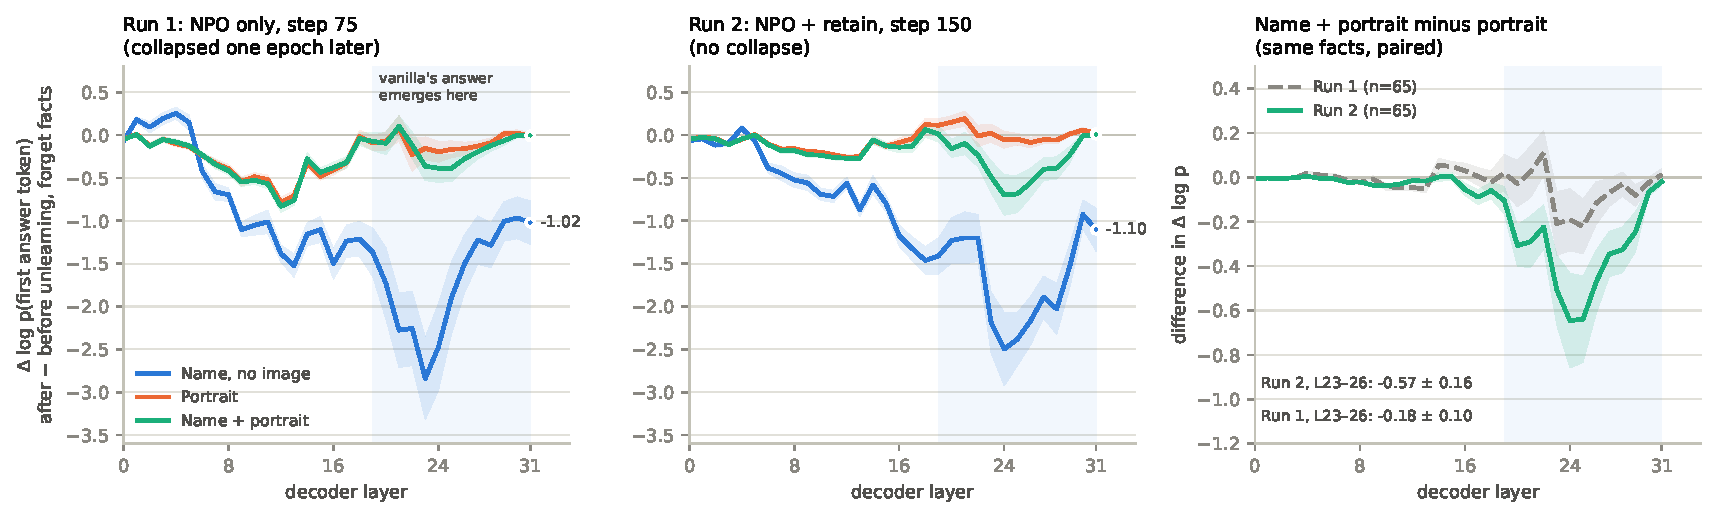
\includegraphics[width=\linewidth]{figures/lens_run1_vs_run2.pdf}
\caption{Logit lens. Change in log probability of the first answer token caused by
unlearning, per decoder layer, on the 65 forget facts. Left: run 1, step 75. Middle: run 2,
step 150. Right: name + portrait minus portrait.}
\label{fig:lens}
\end{figure}

\paragraph{2. Layer masking: which layers carry the forgetting?}
We switch the unlearning LoRA off in a band of layers and check whether the answer to the
name question comes back (Figure~\ref{fig:layer}). The measure is the recovered share of
the lost log probability on the facts the name route lost (24 forget, 8 retain): 0 means
still unlearned, 1 means back to the vanilla. Switching off layers 0--9 recovers 0.96 and
layers 10--19 recovers 0.92; switching off layers 20--31 recovers 0.08. Keeping the LoRA on
in a single band alone produces almost none of the suppression. The effective update is in
layers 0--19, so \textbf{H1 is rejected}.

\begin{figure}[htbp]
\centering
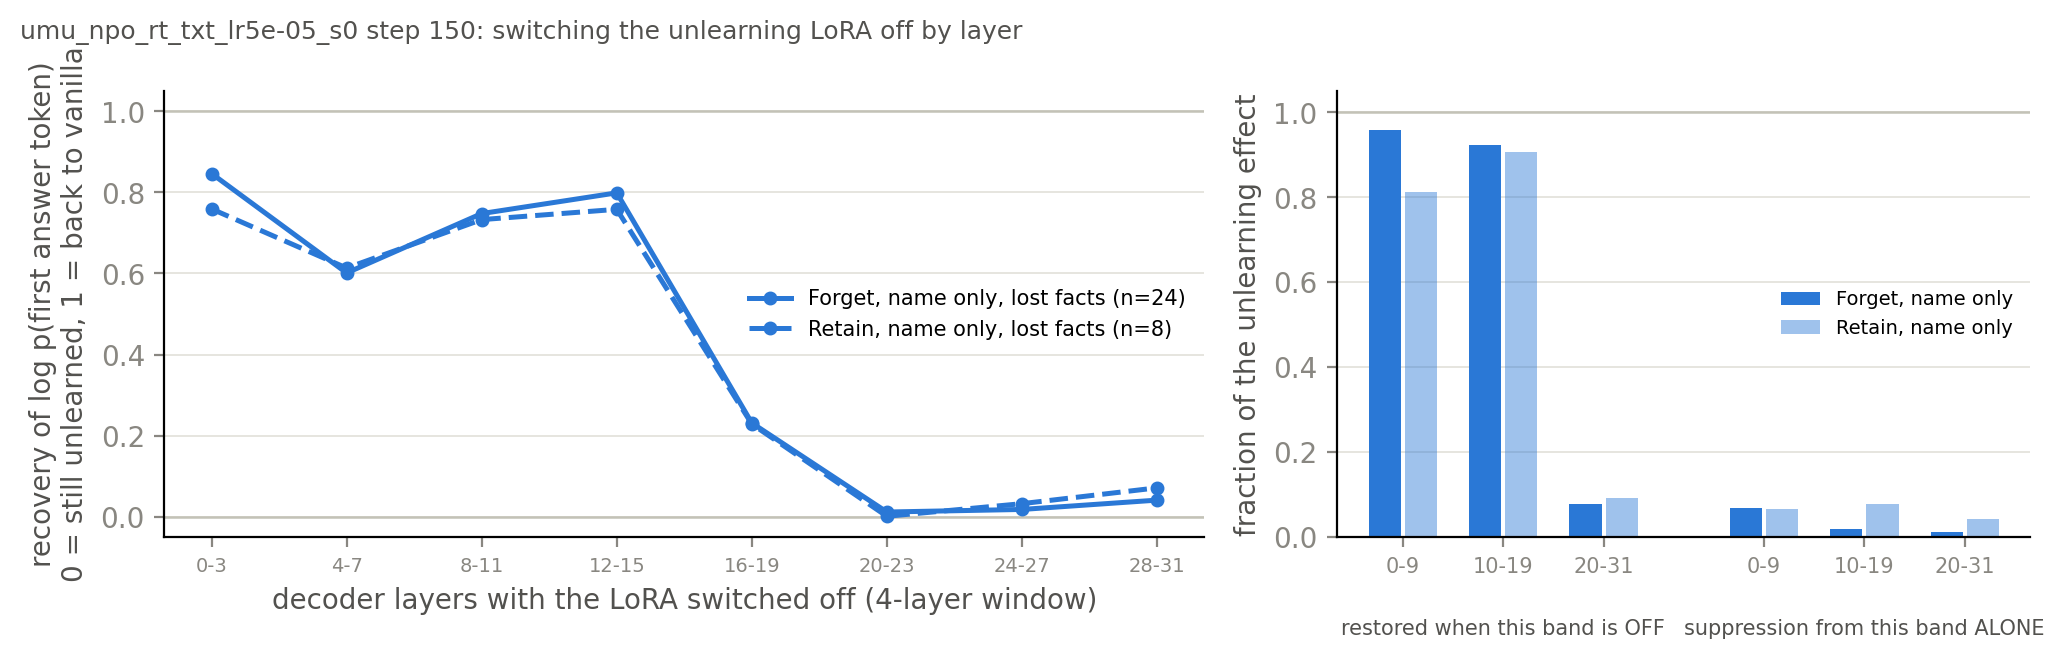
\includegraphics[width=\linewidth]{figures/layer_mask_run2_step150.png}
\caption{Layer masking. Left: LoRA off in one 4-layer window at a time. Right: LoRA off in
a whole band, and LoRA kept on in one band alone.}
\label{fig:layer}
\end{figure}

\paragraph{3. \dwx: how large is the update, and on which tokens?}
For every layer we measure the size of the change the LoRA makes at each token, grouped
into name tokens, image tokens, the rest of the prompt, and the last prompt token
(Figure~\ref{fig:dwx}). The change peaks in layers 8--18 on the name and last tokens, and
is largest of all in layers 28--31, where masking found no effect. It is the same on the
names of forget people and of retain people. No layer writes against the direction of the
correct answer. The size of the update therefore does not show where it matters, and the
update does not distinguish the people it was meant to forget.

\begin{figure}[htbp]
\centering
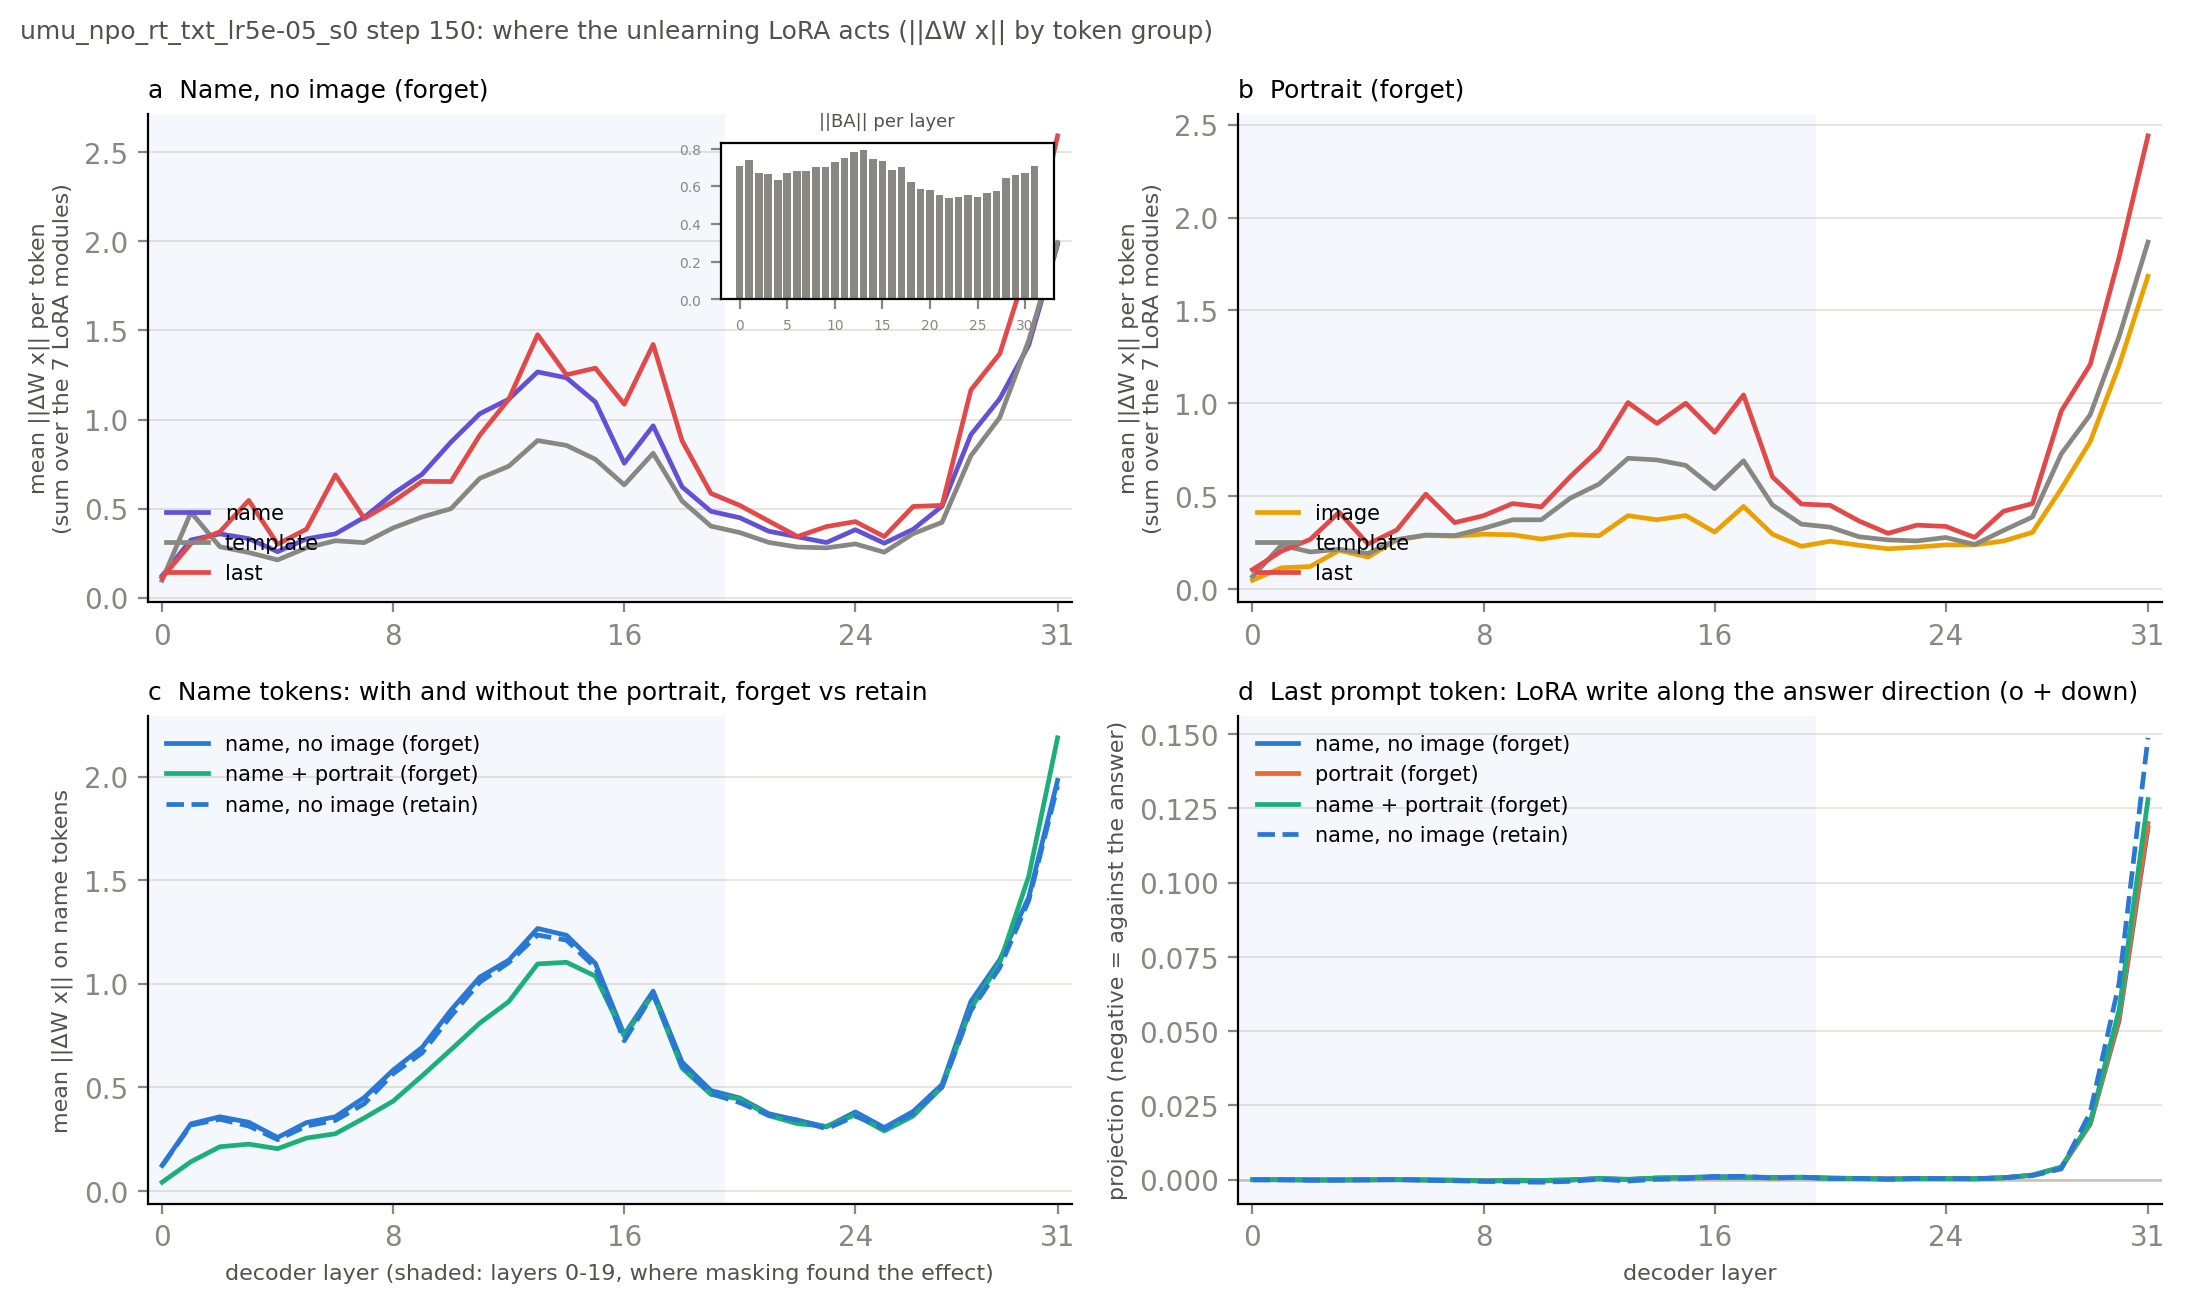
\includegraphics[width=0.92\linewidth]{figures/delta_wx_run2_step150.png}
\caption{Size of the LoRA change per token group and layer. (a) Name question. (b)
Portrait question. (c) Name tokens, with and without the portrait, forget and retain. (d)
Component of the change along the answer direction at the last prompt token.}
\label{fig:dwx}
\end{figure}

\paragraph{4. Position masking: is the update tied to the name?}
We switch the LoRA off only at chosen token positions, in every layer
(Figure~\ref{fig:pos}). The switch is exact: all positions on reproduces $\thu$ and all
positions off reproduces $\tho$. Switching it off at the name tokens recovers 0.37; at the
last prompt token, 0.88; at the rest of the prompt, 0.97. Keeping it on at any one group
alone produces almost no forgetting. The update is spread over the whole text prompt. The
early-to-middle location that \Hp{} proposed holds, but its claim that the change is a
``name pathway'' does not.

\begin{figure}[htbp]
\centering
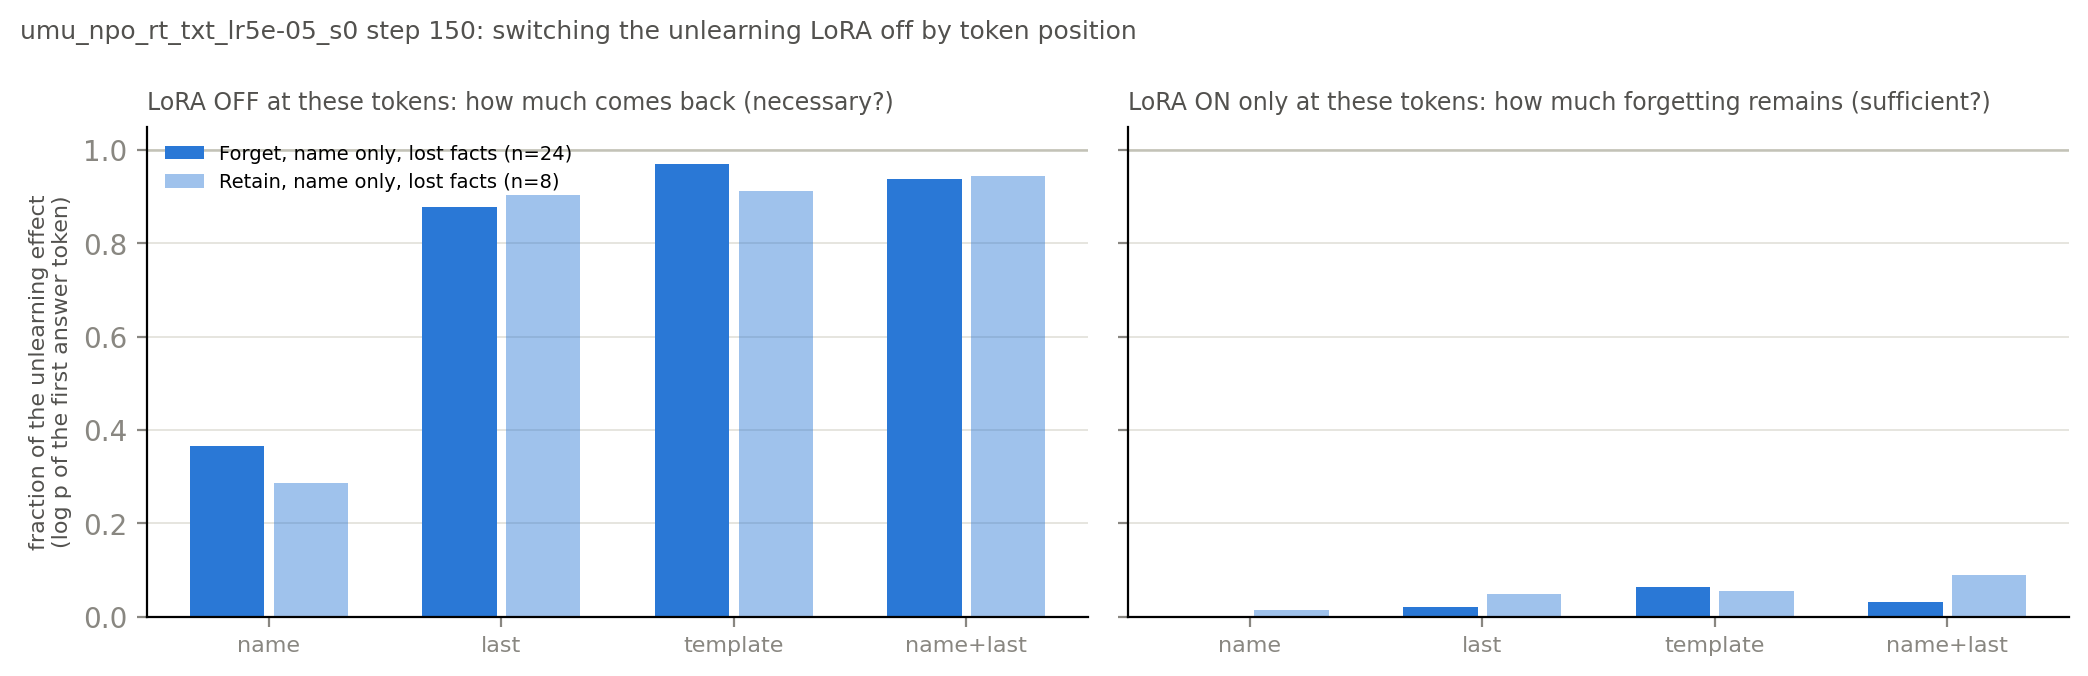
\includegraphics[width=\linewidth]{figures/position_mask_run2_step150.png}
\caption{Position masking on the facts the name route lost (24 forget, 8 retain). Left:
LoRA off at the listed tokens. Right: LoRA on only at the listed tokens.}
\label{fig:pos}
\end{figure}

\paragraph{5. Query-form sweep: which part of the question does the forgetting depend on?}
After analyses 1--4 we formed a new hypothesis, \textbf{H-Q}: text-only unlearning installs
a suppression in layers 0--19 that depends on the form of the text query. It spreads to
other people asked in the same form, and it does not follow the person into other forms.
H-Q was formed after seeing the data, so we fixed five predictions with thresholds before
testing it.

The test starts from the training form (the name question, no options, no image) and
changes one component at a time: image context, how the person is named, wording, answer
format, chat frame (16 forms). For a form $v$,
$F_v=\mathbb{E}[\log p_{\tho}(y\mid v)-\log p_{\thu}(y\mid v)]$ is the drop in the log
probability of the correct answer, and $R_v=1-F_v/F_{\text{train}}$ is the recovery: 0
means as forgotten as in the training form, 1 means unaffected. Figure~\ref{fig:sweep}
shows $R$ for every form and Table~\ref{tab:pred} the outcome of the predictions.

\begin{figure}[htbp]
\centering
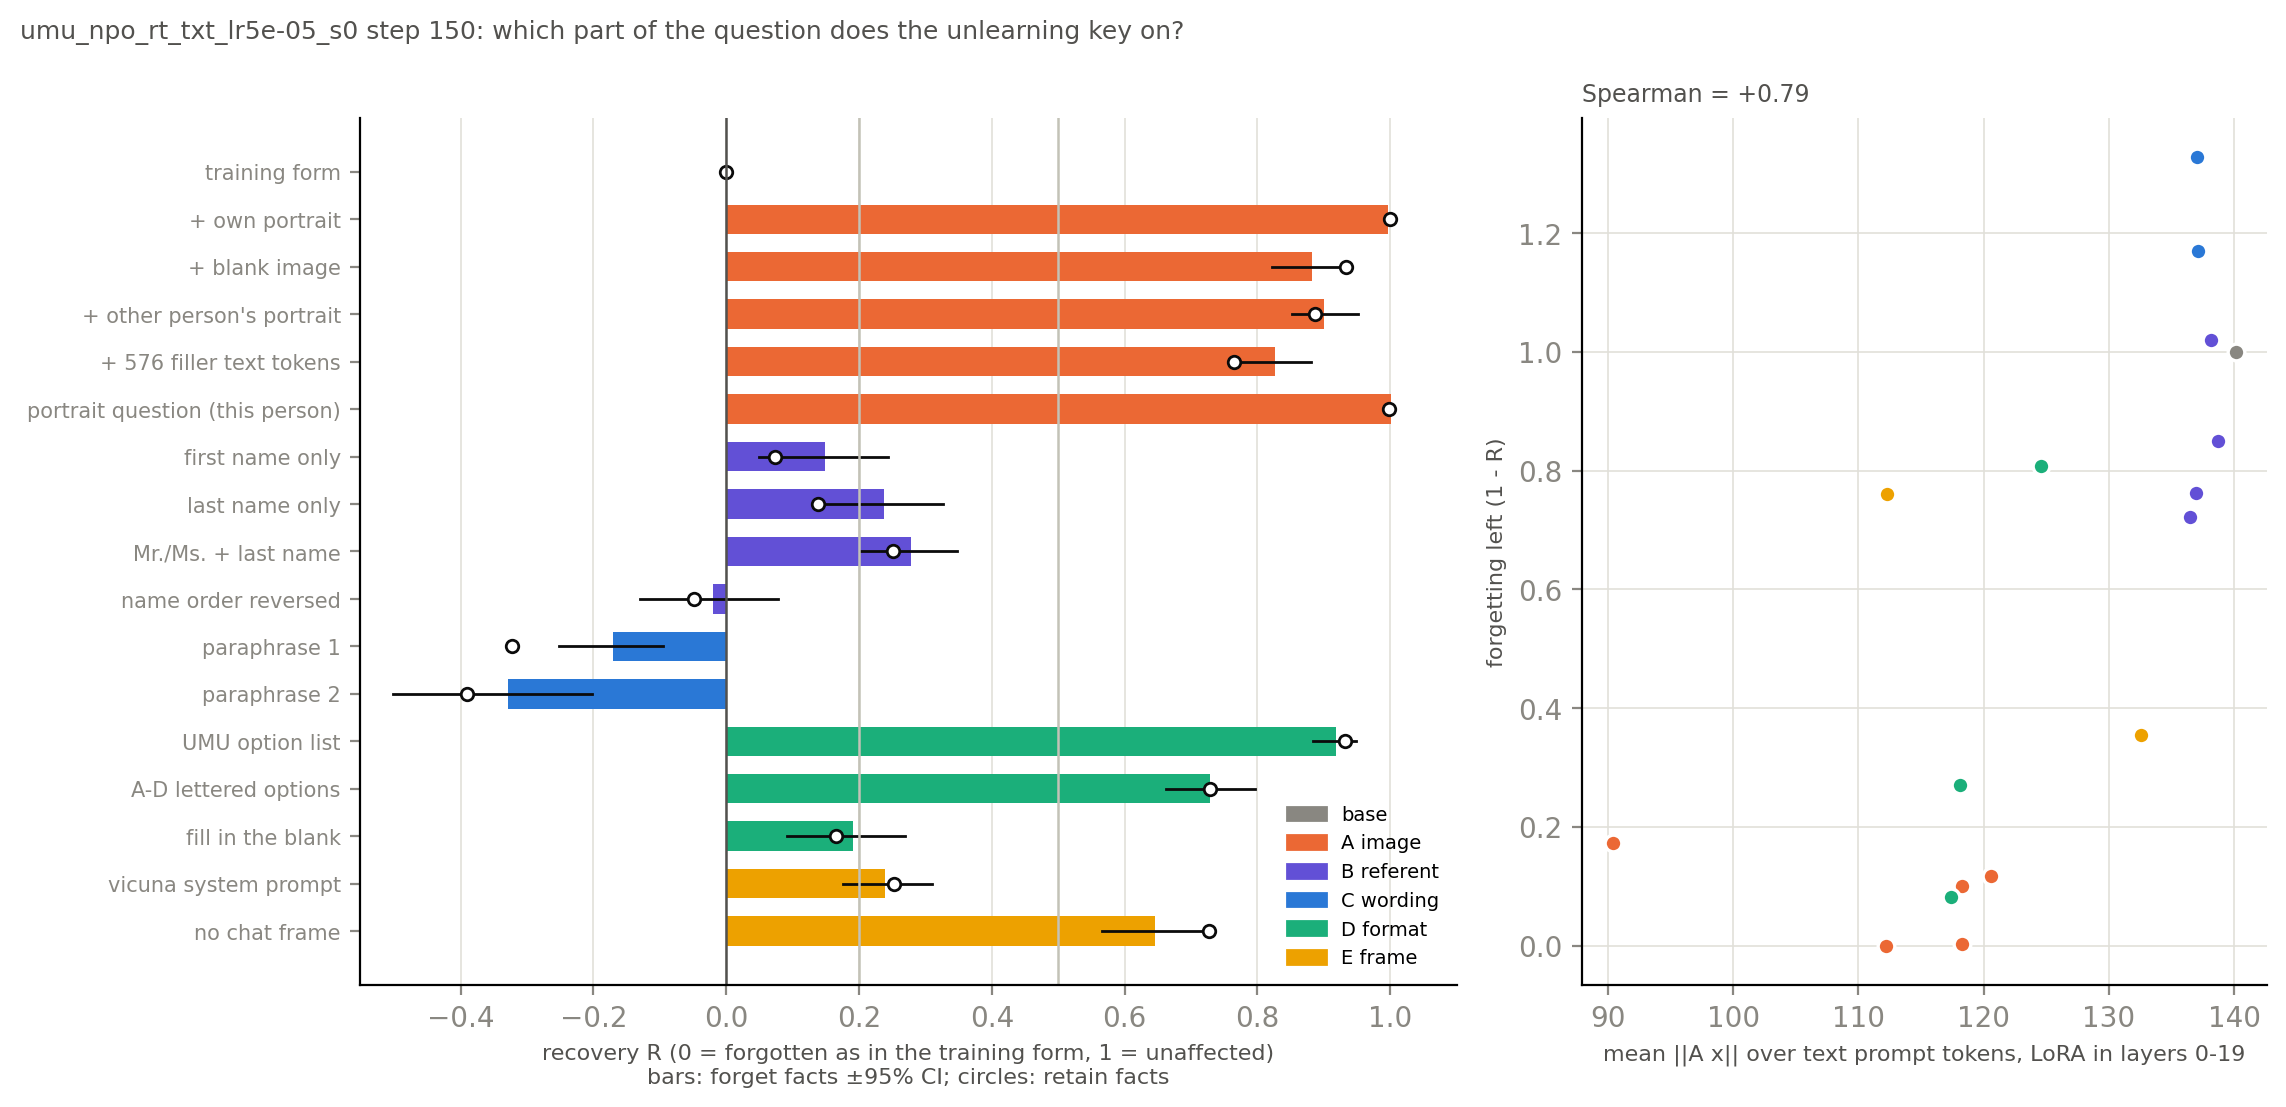
\includegraphics[width=\linewidth]{figures/form_sweep_run2_step150.png}
\caption{Query-form sweep. Left: recovery $R$ per form; bars are forget facts with 95\%
intervals, circles are retain facts. Right: LoRA input activation in layers 0--19 against
the forgetting that remains.}
\label{fig:sweep}
\end{figure}

\begin{table}[htbp]
\centering\small
\begin{tabularx}{\linewidth}{@{}lXXl@{}}
\toprule
 & Prediction (fixed before the run) & Result & Outcome\\
\midrule
P1 & Form, not identity: blank image and 576 filler text tokens each give $R\ge0.5$. &
Blank image 0.88, filler text 0.83 (own portrait 1.00, another person's portrait 0.90). &
Pass\\
P2 & How the name is written does not matter: first name only, last name only and
``Mr./Ms.\ + last name'' each give $R\le0.2$. & 0.15, 0.24, 0.28. & Fail (narrowly)\\
P3 & Not only modality: at least one text-only change gives $R\ge0.3$. & Option list 0.92,
A--D letters 0.73, no chat frame 0.65; paraphrases $-0.17$ and $-0.33$. & Pass\\
P4 & Collateral damage follows the form: Spearman correlation of $R$ on retain and on
forget facts $\ge0.7$. & 0.98 over 16 forms. & Pass\\
P5 & Mechanism matches behaviour: Spearman correlation of LoRA input activation in layers
0--19 with $1-R$ $\ge0.6$. & 0.77. & Pass\\
\bottomrule
\end{tabularx}
\caption{Pre-registered predictions for H-Q and their outcome on run 2, step 150.}
\label{tab:pred}
\end{table}

A blank image carries no information about the person, yet it restores most of the answer
probability. Generation agrees: accuracy falls from 0.77 to 0.37 in the training form but
only from 0.75 to 0.69 with a blank image. Two results in the sweep should not be relied
on yet:
\begin{itemize}
\item The option formats (P3) contain the answer text in the prompt, so the model may copy
it. A control without the answer is missing.
\item Filler text recovers the log probability ($R=0.83$) but only part of the generation
accuracy (0.71 to 0.48). The blank image is the only form without a portrait that escapes
on both readouts, so ``any prefix escapes'' is not established.
\end{itemize}

\paragraph{6. Contribution transplant: does the image stop the suppression from being written?}
The name question with and without a blank image ends in the same tokens (on average 14.4
prompt tokens: the question after its first word, and ``ASSISTANT:''). The LoRA weights
are identical in the two runs, so what the LoRA adds at these tokens can differ only
because the hidden states it reads differ. We record what every LoRA module adds at the
shared tokens in each run, and then swap: the name question runs with the additions
recorded with the image, and the name question with the image runs with the additions
recorded without it. The swap is exact: swapping a prompt's own additions back in changes
the log probability by 0.00.

Two readings were fixed before the run, for layers 0--19. The measure is the moved
fraction $M$: the share of the gap in suppression between the two prompts that follows the
swap. ``The image changes what is written'' requires $M\ge0.5$ in both directions; ``the
same thing is written but not used'' requires $M\le0.2$ in both directions.

On the 65 forget facts, $M=0.41$ (95\% interval 0.34--0.48) when the name question
receives the additions recorded with the image, and $M=0.06$ (0.03--0.09) when the prompt
with the image receives the additions recorded without it
(Figure~\ref{fig:transplant}). By the fixed rule this is a mixed outcome: neither reading
holds in both directions. In layers 20--31, the control, the swap does nothing
($|M|<0.01$). Table~\ref{tab:transplant} gives the same result as suppression in each
prompt.

\begin{table}[htbp]
\centering\small
\begin{tabular}{@{}lccc@{}}
\toprule
 & \multicolumn{3}{c}{What the LoRA adds at the shared tokens in layers 0--19}\\
\cmidrule(l){2-4}
Prompt & recorded without image & recorded with image & nothing\\
\midrule
Name question & 14.42 & 9.24 & 0.76\\
Name question + blank image & 2.40 & 1.68 & 0.63\\
\bottomrule
\end{tabular}
\caption{Suppression of the correct answer: drop in log probability relative to the
vanilla, in nats, on 65 forget facts. 14.42 and 1.68 are the unmodified runs.}
\label{tab:transplant}
\end{table}

\begin{figure}[htbp]
\centering
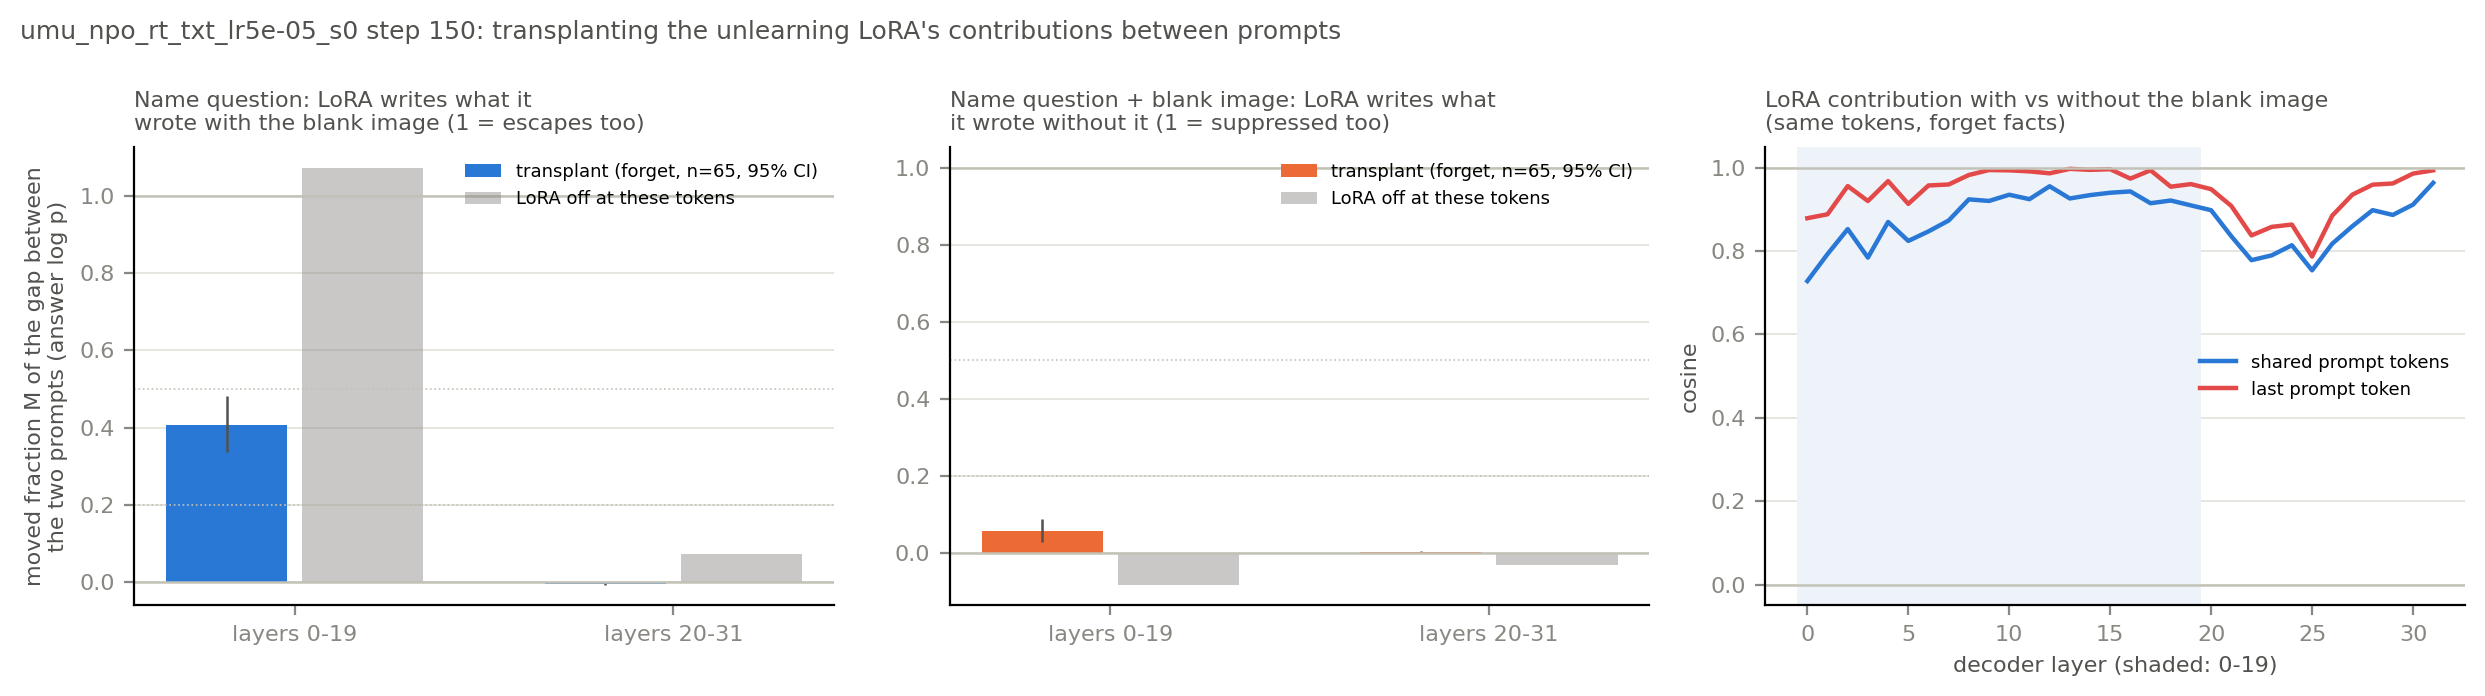
\includegraphics[width=\linewidth]{figures/transplant_run2_step150.png}
\caption{Contribution transplant. Left and middle: moved fraction $M$ per layer band, with
the LoRA switched off at the same tokens as a reference. Right: cosine between what the
LoRA adds with and without the image, per layer.}
\label{fig:transplant}
\end{figure}

The table supports three statements.
\begin{itemize}
\item \textbf{The image does not stop the write.} The additions recorded without the
image carry 14.4 nats of suppression in their own prompt, but add only 0.7 nats when
written into the prompt with the image (2.40 against 1.68).
\item \textbf{What is written is similar in both cases.} In layers 0--19 the cosine
between the two sets of additions averages 0.89 on the shared prompt tokens and 0.96 at
the last prompt token.
\item \textbf{The write still matters.} The additions recorded with the image carry 9.2 of
the 14.4 nats in the name question.
\end{itemize}
Suppression therefore needs both the additions of the text-only run and a text-only
prompt, and the prompt is the larger factor. This reading was formed after seeing the
data. Two limits apply. Foreign additions may disturb a run in ways unrelated to
forgetting; this can only raise the two swapped values, so 2.40 is an upper bound and the
first statement is safe, but 9.24 may overstate what the additions recorded with the image
suppress. One token per fact, the first word of the question, is tokenised differently
after the image and keeps its own additions.

The same test on the retain facts and on a second checkpoint from a different recipe
(run~1, NPO without a retain term, step 75) gives the same asymmetry
(Table~\ref{tab:transplantrep}). In all four cases the additions recorded without the
image add no suppression in the prompt with the image ($M$ between $-0.03$ and $0.06$),
and the outcome under the fixed rule is mixed.

\begin{table}[htbp]
\centering\small
\begin{tabular}{@{}lcccc@{}}
\toprule
 & Forgetting, name / + image (nats) & $R$ & $M$, name question & $M$, name + image\\
\midrule
Run 2, forget (65) & 14.42 / 1.68 & 0.88 & 0.41 [0.34, 0.48] & 0.06 [0.03, 0.09]\\
Run 2, retain (26) & 12.08 / 0.82 & 0.93 & 0.43 [0.31, 0.52] & 0.06 [0.03, 0.10]\\
Run 1, forget (65) & 5.90 / 1.55 & 0.74 & 0.64 [0.45, 0.81] & $-0.03$ [$-0.05$, $-0.01$]\\
Run 1, retain (26) & 5.60 / 0.55 & 0.90 & 0.55 [0.30, 0.75] & $-0.02$ [$-0.04$, $-0.00$]\\
\bottomrule
\end{tabular}
\caption{Contribution transplant in layers 0--19 on two checkpoints. $M$ with 95\%
intervals; ``name question'' is the name question receiving the additions recorded with
the image, ``name + image'' the reverse.}
\label{tab:transplantrep}
\end{table}

\section{Where this leaves the hypotheses}
\begin{itemize}
\item \textbf{H2 rejected:} the portrait route is not suppressed and repaired.
\item \textbf{H1 rejected:} the late layers are neither necessary nor sufficient.
\item \textbf{\Hp{} half right:} the update is in the early and middle layers, but it is
not bound to the name tokens.
\item \textbf{H-Q supported so far:} forgetting depends on the form of the input. The leak
to portrait questions and the damage to other people asked by name are two consequences of
the same thing.
\end{itemize}
What we can state is where the update acts and what it depends on. On \emph{why} an image
bypasses it, the transplant gives a partial answer: the update is still written when an
image is present, and it takes effect only in a text-only prompt. We cannot yet state what
in the image context makes it ineffective, or why NPO arrives at this solution.

\section{Not done, and limits}
\begin{itemize}
\item \textbf{Written but without recorded results:} the blank-image route patching
(\texttt{scripts/mech\_umu\_blank\_patch.py}), the input-cue experiment
(\texttt{scripts/mech\_umu\_input\_cues.py}: blank image before or after the question,
blank image with zeroed features, text prefixes of several lengths), and run~4 (lr
$10^{-4}$ with the strong retain term).
\item \textbf{One checkpoint, one seed.} The logit lens and the contribution transplant
were also run on a second checkpoint (run~1, step 75); for the other analyses we have
recorded results on this checkpoint only.
\item \textbf{Small samples.} Layer and position masking use 24 forget and 8 retain facts
and report no confidence intervals.
\item \textbf{One method, one model, one direction.} Only NPO on LLaVA-1.5-7B with
text-only unlearning. Image-only unlearning was not run, so the asymmetry between the two
directions, part of the original question, is not addressed.
\item \textbf{Fictitious, fine-tuned knowledge.} The facts were injected by fine-tuning and
may be stored differently from knowledge acquired in pretraining. The vanilla never saw an
input without an image, which may make the no-image form unusual in itself.
\item \textbf{Weak unlearning.} The analysed checkpoint forgets 37\% of the forget facts by
name and damages 31\% of the retain facts.
\item \textbf{References.} Entries marked \texttt{VERIFY} in the source of this file come
from our notes and have not been checked against the papers.
\end{itemize}

\begin{thebibliography}{99}\small
\bibitem{umubench} C.~Wang, Y.~Li, X.~Feng, C.~Chen, X.~Zheng, J.~Yin.
  UMU-Bench: Closing the Modality Gap in Multimodal Unlearning Evaluation. NeurIPS 2025 Datasets and Benchmarks Track.
\bibitem{mllmu} Z.~Liu et al. Protecting Privacy in Multimodal Large Language Models with MLLMU-Bench.
  arXiv:2410.22108. % VERIFY author list and venue
\bibitem{llava15} H.~Liu, C.~Li, Y.~Li, Y.~J.~Lee. Improved Baselines with Visual Instruction Tuning. arXiv:2310.03744.
\bibitem{npo} R.~Zhang, L.~Lin, Y.~Bai, S.~Mei. Negative Preference Optimization: From Catastrophic Collapse to
  Effective Unlearning. arXiv:2404.05868.
\bibitem{unlinkvl} UNLINK-VL. arXiv:2608.03791. % VERIFY: full title and authors (research.md notes inconsistent author lists)
\bibitem{smu} SMU. arXiv:2607.18615. % VERIFY full reference
\bibitem{idunlearn} IDUnlearn-Bench. arXiv:2609.33481. % VERIFY full reference
\bibitem{crossinf} CrossInf. arXiv:2607.16442. % VERIFY full reference
\bibitem{pava} PAVA. arXiv:2608.30649. % VERIFY full reference
\bibitem{hong2024} Y.~Hong et al. Intrinsic evaluation of unlearning using parametric knowledge traces.
  arXiv:2406.11614. % VERIFY: research.md cites 2410.06606 (MLP coefficients) and 2406.11614 (ConceptVectors)
\bibitem{guo2024} P.~Guo et al. Mechanistic unlearning: robust knowledge unlearning and editing via mechanistic
  localization. arXiv:2410.12949. % VERIFY
\end{thebibliography}

\end{document}
